\chapter{Module Data Science et Intelligence Artificielle}

\section{Introduction}

Ce chapitre présente la contribution Data Science et Intelligence Artificielle intégrée à la plateforme \textbf{Virtual FabLab}. Contrairement au chapitre précédent, centré sur la réalisation logicielle, cette partie analyse la chaîne de traitement des données, les modèles utilisés, le classifieur d'intentions et le copilote d'aide à la décision réservé à l'administrateur.

Le module étudié repose sur des données de télémétrie simulées. Il ne constitue donc pas une validation industrielle de maintenance prédictive, mais un prototype académique permettant de démontrer l'intégration entre ingestion MQTT, stockage, apprentissage automatique, classification supervisée d'intentions et restitution des résultats dans l'interface d'administration.

\section{Architecture du module Data Science et IA}

Le module Data Science et IA est placé côté backend. Il reçoit les mesures stockées après ingestion MQTT, extrait les caractéristiques nécessaires, charge les modèles persistés avec \texttt{joblib}, puis produit des résultats structurés consommés par le tableau de bord et par le Copilote IA de maintenance.

\begin{figure}[H]
\centering
\IfFileExists{images/architecture_data_science_ia.png}
{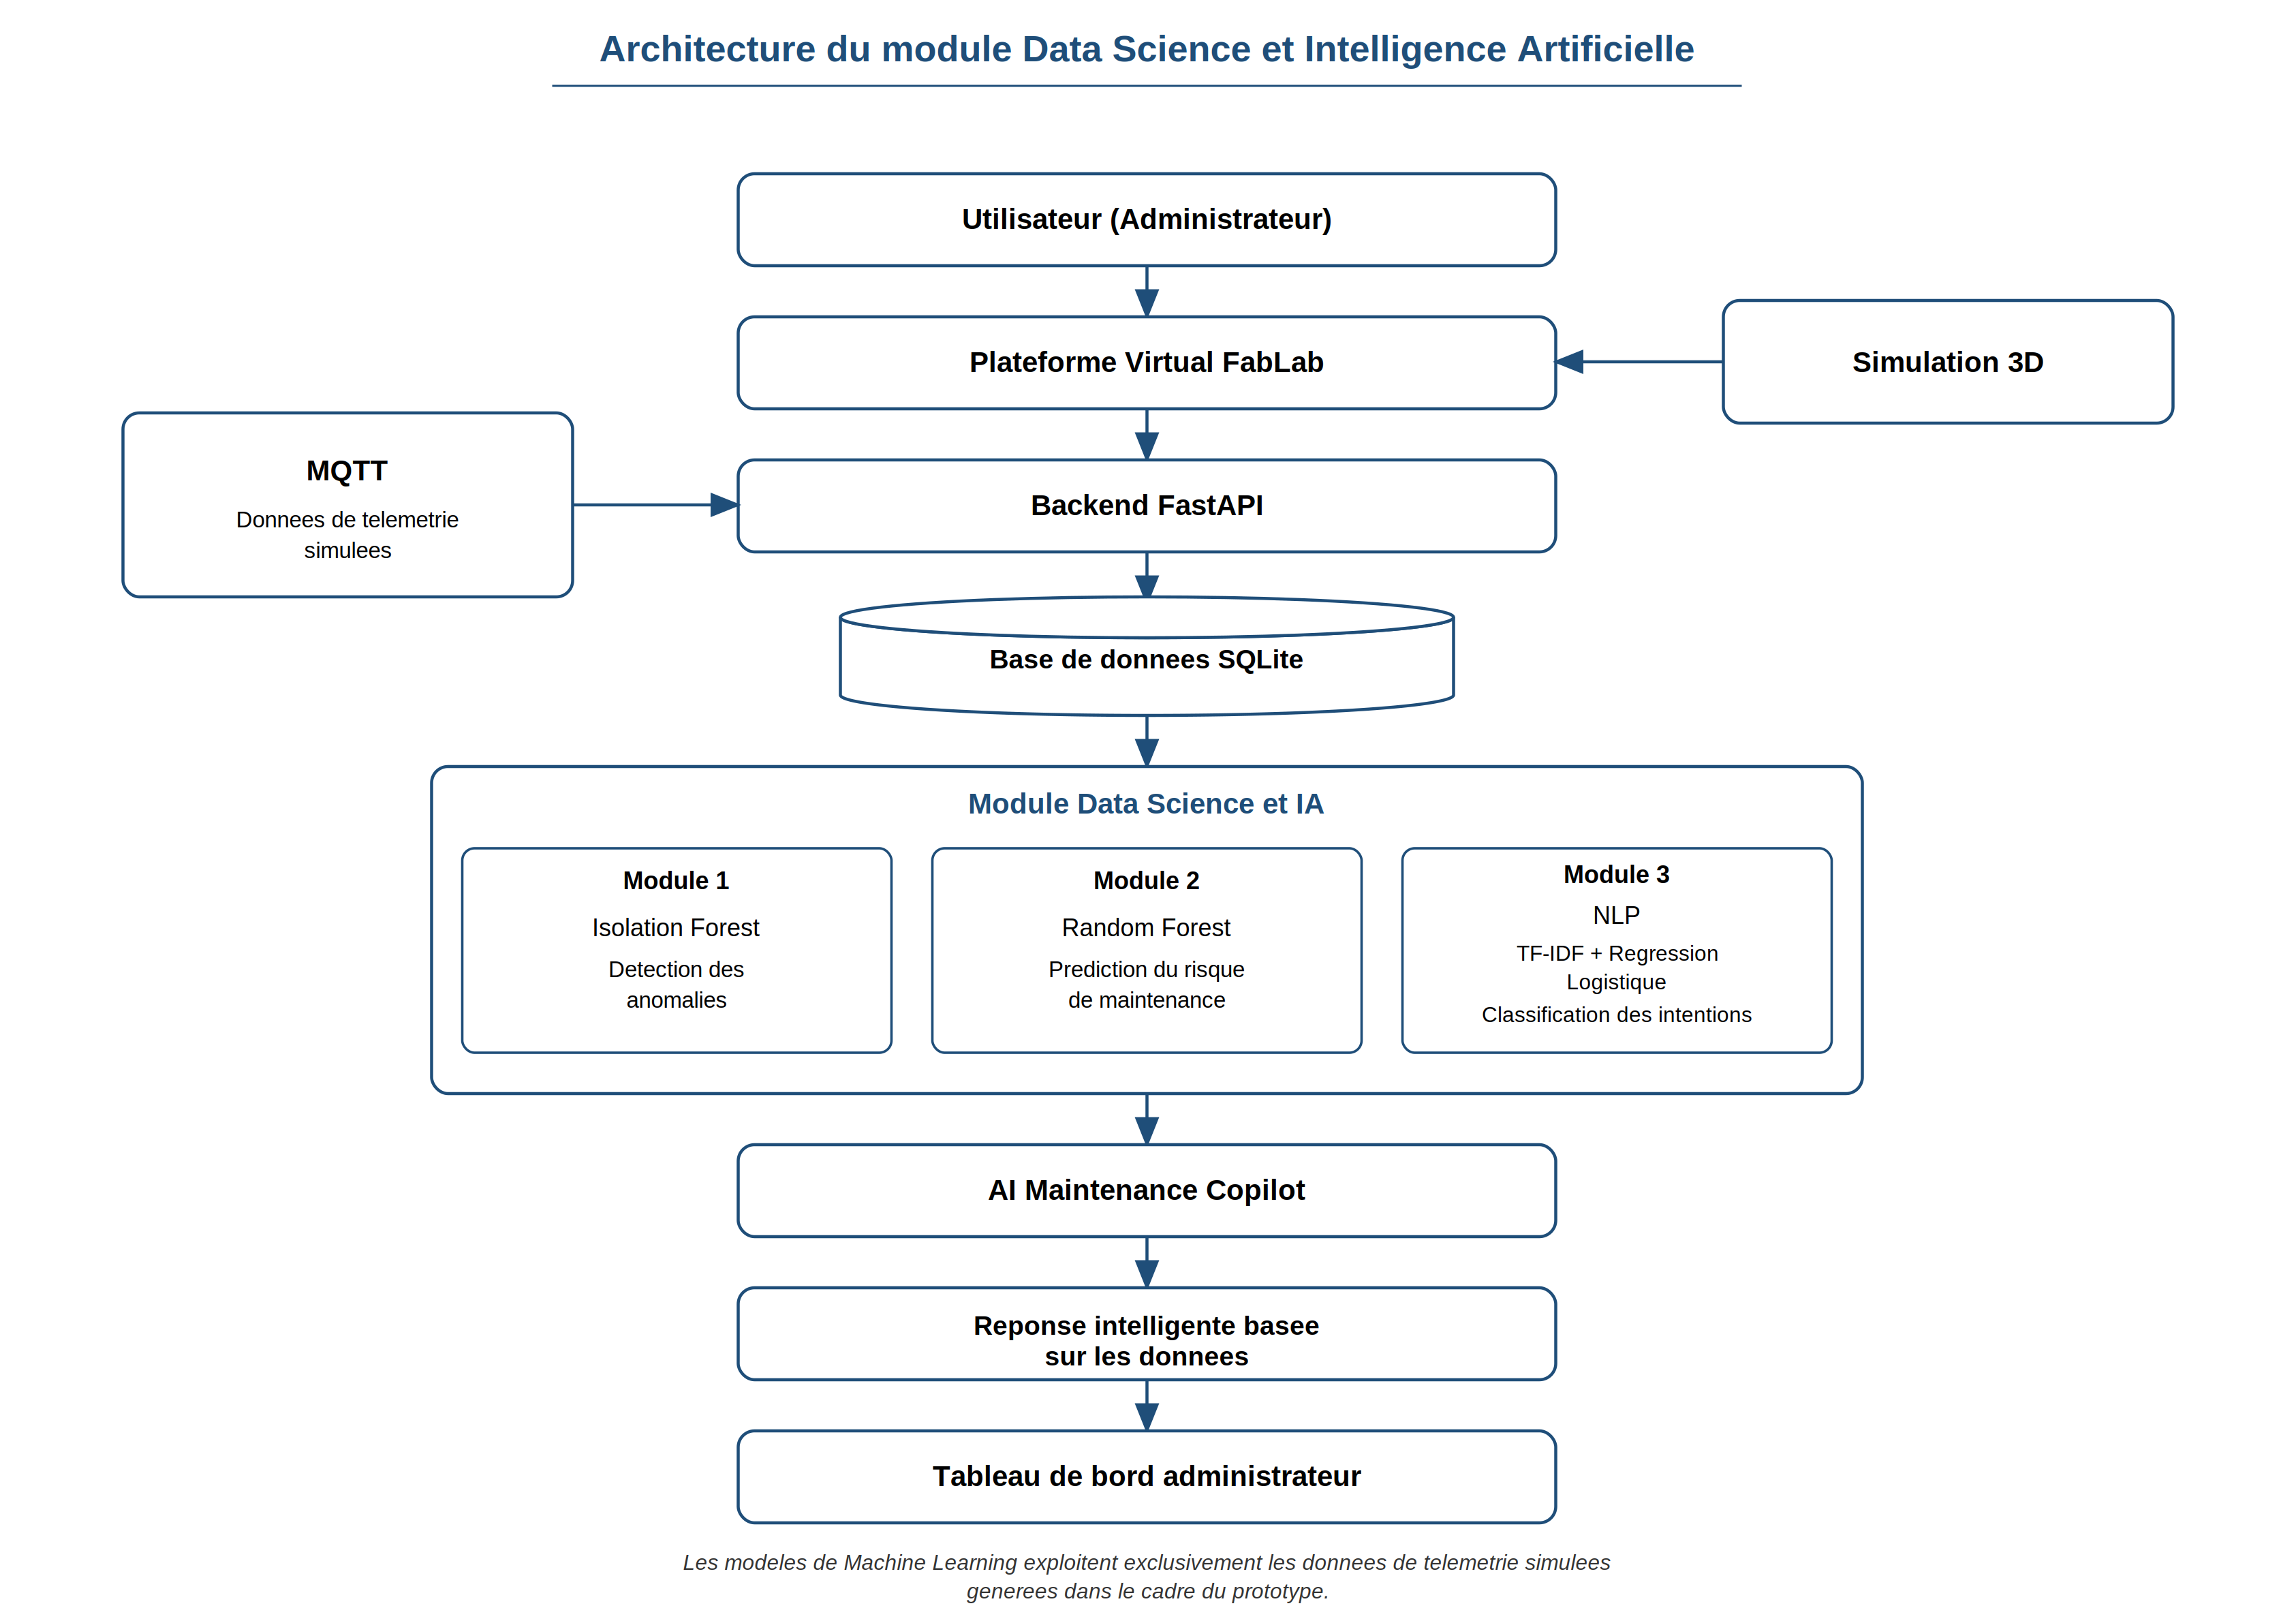
\includegraphics[width=0.95\textwidth]{images/architecture_data_science_ia.png}}
{\fbox{\parbox[c][5.8cm][c]{0.88\textwidth}{\centering Emplacement réservé pour le pipeline Data Science et IA\\[2mm]\texttt{images/architecture\_data\_science\_ia.png}\\[2mm]\small MQTT telemetry $\rightarrow$ database $\rightarrow$ preprocessing $\rightarrow$ feature engineering $\rightarrow$ Isolation Forest $\rightarrow$ Random Forest $\rightarrow$ health/risk outputs $\rightarrow$ dashboard and Copilot}}}
\caption{Pipeline Data Science et IA de la plateforme}
\label{fig:architecture-data-science-ia}
\end{figure}

La figure \ref{fig:architecture-data-science-ia} doit représenter le passage des messages MQTT vers la base de données, puis vers les traitements de prétraitement, d'ingénierie des caractéristiques, de détection d'anomalies, d'estimation du risque et de restitution dans le tableau de bord et le copilote.

\section{Collecte et nature des données}

Les données exploitées par le module proviennent d'un simulateur MQTT, et non de capteurs physiques connectés. Le script de simulation publie des messages JSON sur des topics propres à chaque machine, selon le motif suivant :

\begin{center}
\small\texttt{fablab/machines/\{machine\_id\}/data}
\end{center}

Le backend s'abonne au motif \texttt{fablab/machines/+/data}, parse les messages reçus et enregistre les mesures dans la table des lectures capteurs.

Les champs effectivement exploités sont la température, la vibration, la durée d'utilisation, la vitesse du moteur, l'erreur éventuelle et l'horodatage. La durée d'utilisation est reçue sous forme de \texttt{usage\_duration}, puis convertie en heures pour les modèles. La présence d'une erreur est transformée en variable binaire.

\begin{table}[H]
\centering
\small
\caption{Nature des données utilisées par le module Data Science}
\label{tab:donnees-ds-ia}
\begin{tabular}{|p{0.24\textwidth}|p{0.22\textwidth}|p{0.44\textwidth}|}
\hline
\rowcolor{SectionColor!12}
\textbf{Donnée} & \textbf{Origine} & \textbf{Utilisation} \\
\hline
\texttt{temperature} & MQTT simulé & Détection de dérive thermique, score de risque et facteurs explicatifs. \\
\hline
\texttt{vibration} & MQTT simulé & Détection de vibration anormale et estimation du risque. \\
\hline
\texttt{motor\_speed} & MQTT simulé & Contrôle de cohérence et contribution au risque. \\
\hline
\texttt{usage\_duration} & MQTT simulé & Conversion en \texttt{usage\_hours} pour les modèles et le score de maintenance. \\
\hline
\texttt{error} & MQTT simulé & Historique d'erreurs et variable binaire \texttt{has\_error}. \\
\hline
\texttt{timestamp} & MQTT simulé & Ordonnancement temporel et analyse de fraîcheur des mesures. \\
\hline
\end{tabular}
\end{table}

\section{Prétraitement des données}

Le prétraitement est volontairement limité et cohérent avec l'état actuel du code. Lors de l'ingestion, les messages JSON sont validés par un schéma Pydantic avant d'être persistés. Pour l'entraînement des modèles Machine Learning, le script \texttt{train\_ml\_models.py} convertit les colonnes numériques en valeurs exploitables, remplace les valeurs manquantes par zéro pour les colonnes attendues et calcule la variable \texttt{has\_error} à partir du champ \texttt{error}.

La conversion temporelle principale consiste à transformer \texttt{usage\_duration} en \texttt{usage\_hours}. Le code ne met pas en évidence une normalisation ou une standardisation explicite des variables numériques pour les modèles Isolation Forest et Random Forest. Le rapport ne doit donc pas affirmer l'existence d'une mise à l'échelle qui n'est pas implémentée.

Pour les analyses temps réel, les lectures récentes sont récupérées en ordre décroissant d'horodatage, avec une limite de 48 points pour l'évaluation de maintenance et une fenêtre configurable pour le contexte du copilote.

\section{Ingénierie des caractéristiques}

Les caractéristiques utilisées par les modèles persistés sont définies dans les métadonnées du dossier \texttt{backend/ml\_models}. Elles sont les suivantes : \texttt{temperature}, \texttt{vibration}, \texttt{usage\_hours}, \texttt{motor\_speed} et \texttt{has\_error}.

\begin{table}[H]
\centering
\small
\caption{Entrées utilisées par les modèles Machine Learning}
\label{tab:features-modeles}
\begin{tabular}{|p{0.27\textwidth}|p{0.63\textwidth}|}
\hline
\rowcolor{SectionColor!12}
\textbf{Caractéristique} & \textbf{Description} \\
\hline
\texttt{temperature} & Température de fonctionnement issue de la télémétrie simulée. \\
\hline
\texttt{vibration} & Niveau de vibration transmis par le simulateur MQTT. \\
\hline
\texttt{usage\_hours} & Durée d'utilisation en heures, dérivée de \texttt{usage\_duration / 60}. \\
\hline
\texttt{motor\_speed} & Vitesse du moteur, exprimée en tours par minute dans l'interface. \\
\hline
\texttt{has\_error} & Variable binaire indiquant la présence d'un code erreur. \\
\hline
\end{tabular}
\end{table}

En complément des modèles, le service prédictif calcule des facteurs explicatifs par règles : contribution de la température, de la vibration, de la durée d'utilisation, des erreurs récentes et d'une tendance simple basée sur l'évolution moyenne de la température et de la vibration. Ces facteurs servent à rendre les résultats plus interprétables dans le tableau de bord et dans les réponses du copilote.

\section{Détection des anomalies par Isolation Forest}

La détection d'anomalies vise à signaler des comportements inhabituels dans les mesures machines. Le modèle utilisé est un \textit{Isolation Forest}, entraîné avec scikit-learn et persisté dans \texttt{backend/ml\_models/anomaly\_isolation\_forest.joblib}.

Le principe d'Isolation Forest consiste à isoler les observations atypiques par des partitions aléatoires. Les points plus faciles à isoler sont considérés comme plus susceptibles d'être anormaux. Dans le script d'entraînement, le modèle est ajusté sur les exemples de classe \texttt{normal}. Les paramètres explicitement vérifiés sont :

\begin{itemize}
    \item \texttt{n\_estimators=180} ;
    \item \texttt{contamination=0.18} ;
    \item \texttt{random\_state=42}.
\end{itemize}

À l'inférence, le service charge le modèle et appelle \texttt{predict} et \texttt{decision\_function}. La sortie \texttt{-1} est interprétée comme une anomalie. Le score retourné est arrondi et exposé dans les réponses de monitoring. Si les fichiers de modèles sont absents ou si une erreur survient, une logique de repli par règles produit une estimation indicative.

Cette détection reste limitée par la nature simulée des données et par l'absence de validation sur machines physiques. Elle doit être interprétée comme une aide à la décision dans le cadre du prototype.

\section{Évaluation du risque de maintenance par Random Forest}

Le risque de maintenance est estimé par un \textit{Random Forest Classifier} scikit-learn, persisté dans \texttt{backend/ml\_models/maintenance\_random\_forest.joblib}. Le modèle est entraîné sur les mêmes caractéristiques que l'Isolation Forest, mais avec une cible supervisée appelée \texttt{maintenance\_label}.

Les classes vérifiées dans les métadonnées sont \texttt{normal}, \texttt{monitor}, \texttt{maintenance\_soon} et \texttt{critical}. Le script d'entraînement utilise des données synthétiques générées par code et un fichier CSV de démonstration, puis effectue une séparation entraînement/test avec \texttt{test\_size=0.22}, \texttt{random\_state=42} et stratification. Les paramètres vérifiés du Random Forest sont \texttt{n\_estimators=220}, \texttt{class\_weight="balanced"} et \texttt{random\_state=42}.

À l'inférence, le service récupère les probabilités de classes avec \texttt{predict\_proba}. Une probabilité indicative de défaillance est calculée par pondération des classes : \texttt{normal} vaut 0,05, \texttt{monitor} vaut 0,30, \texttt{maintenance\_soon} vaut 0,68 et \texttt{critical} vaut 0,95. Le score de santé est ensuite calculé comme \texttt{100 - failure\_probability * 100}, borné entre 0 et 100.

Cette sortie n'est pas une prédiction industrielle validée. Elle correspond à une estimation du risque sur des données simulées et sert à prioriser la surveillance dans l'interface administrateur.

\section{Classification NLP des intentions administrateur}

Le Copilote IA de maintenance utilise une classification supervisée d'intentions. Il ne s'agit pas d'un modèle génératif ni d'un LLM. Le pipeline d'apprentissage est défini dans le script d'entraînement du classifieur et combine un \texttt{TfidfVectorizer} avec une \texttt{LogisticRegression}.

Le prétraitement texte vérifié inclut la conversion en minuscules, la suppression des accents avec \texttt{strip\_accents="unicode"}, l'utilisation de n-grammes de mots de taille 1 et 2, \texttt{min\_df=1}, \texttt{sublinear\_tf=True} et un motif de token compatible avec certains identifiants de machines. Le classifieur Logistic Regression utilise \texttt{max\_iter=1000}, \texttt{class\_weight="balanced"}, \texttt{solver="lbfgs"}, \texttt{C=4.0} et \texttt{random\_state=42}.

Les intentions supportées sont les suivantes :

\begin{itemize}
    \item \texttt{fablab\_summary}, \texttt{machine\_status}, \texttt{explain\_machine\_health} ;
    \item \texttt{highest\_risk\_machine}, \texttt{compare\_machines}, \texttt{recent\_anomalies} ;
    \item \texttt{maintenance\_recommendation}, \texttt{reservation\_summary}, \texttt{help} et \texttt{unknown}.
\end{itemize}

Le modèle est persisté dans le fichier \texttt{copilot\_intent\_classifier.joblib}. À l'inférence, une intention est acceptée seulement si la confiance atteint le seuil \texttt{0.20}; sinon, l'intention devient \texttt{unknown}.

\begin{figure}[H]
\centering
\IfFileExists{images/pipeline_nlp_copilot.png}
{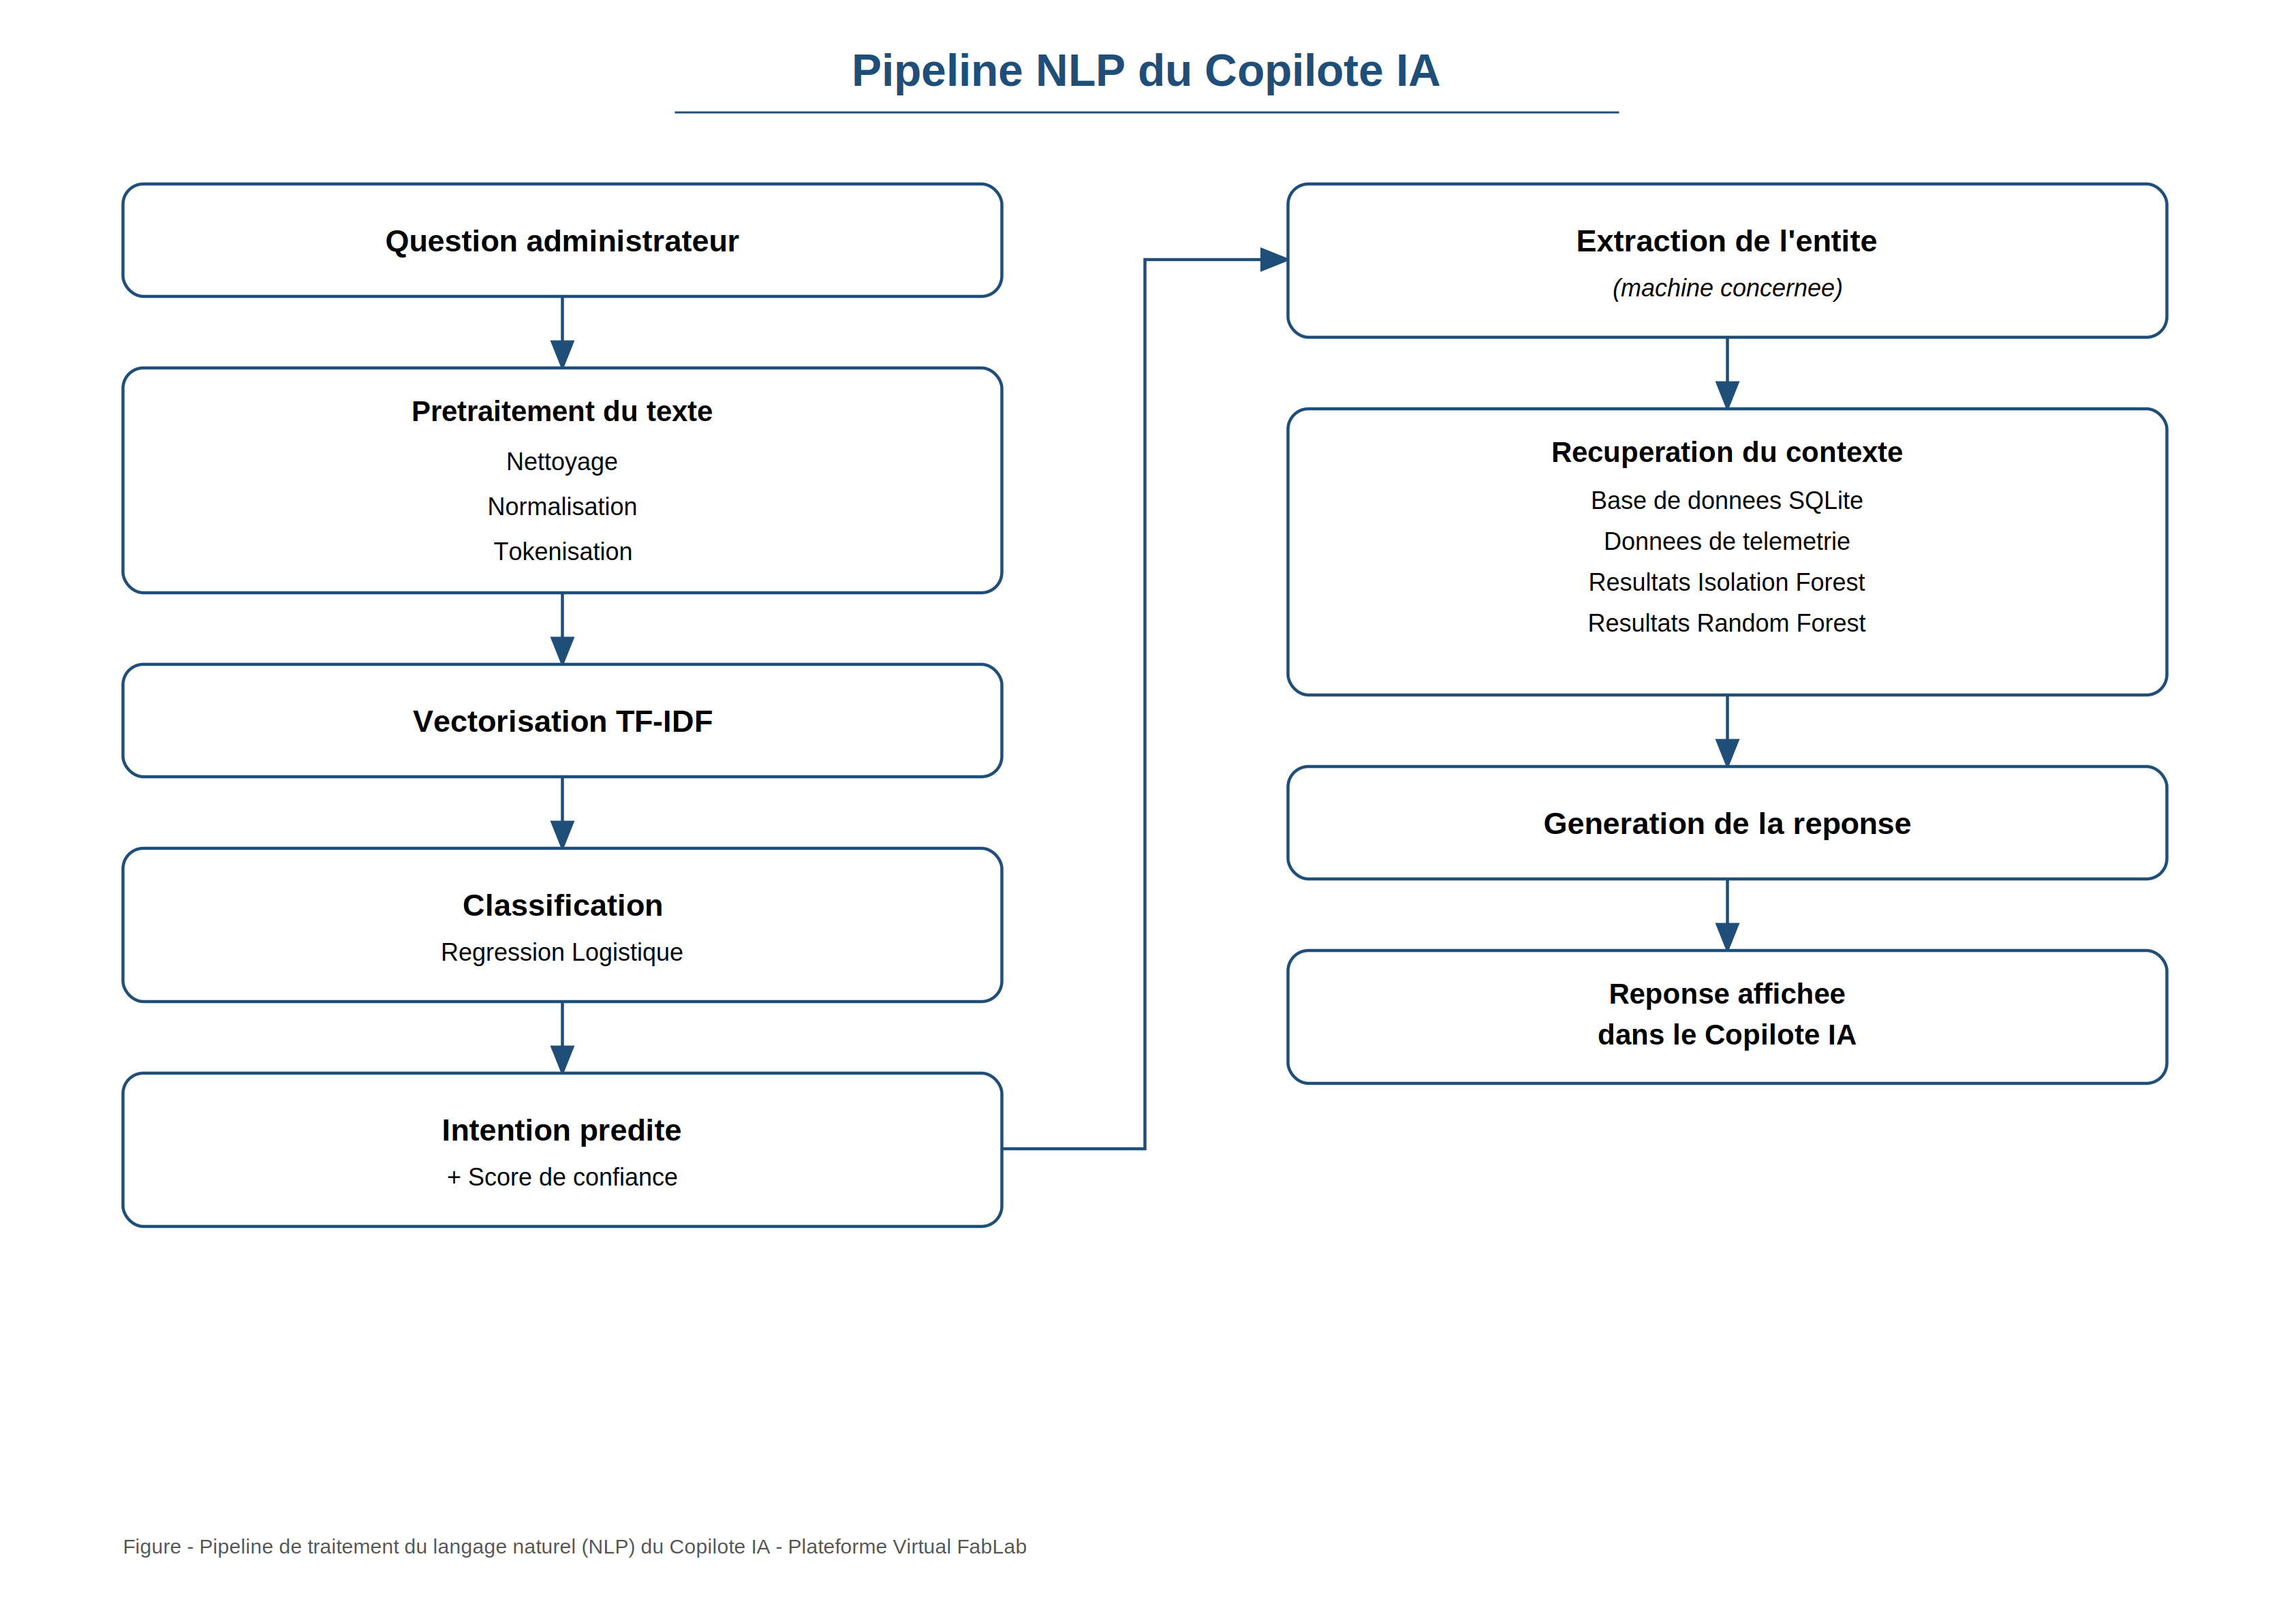
\includegraphics[width=0.95\textwidth]{images/pipeline_nlp_copilot.png}}
{\fbox{\parbox[c][5.8cm][c]{0.88\textwidth}{\centering Emplacement réservé pour le workflow NLP du Copilote\\[2mm]\texttt{images/pipeline\_nlp\_copilot.png}\\[2mm]\small Administrator question $\rightarrow$ text preprocessing $\rightarrow$ TF-IDF $\rightarrow$ Logistic Regression $\rightarrow$ predicted intent and confidence $\rightarrow$ entity extraction $\rightarrow$ telemetry context retrieval $\rightarrow$ ML results $\rightarrow$ grounded response $\rightarrow$ admin interface}}}
\caption{Workflow NLP du Copilote IA de maintenance}
\label{fig:pipeline-nlp-copilot}
\end{figure}

\section{Copilote IA de maintenance}

Le Copilote IA de maintenance est un copilote d'aide à la décision combinant détection d'anomalies, prédiction du risque, classification supervisée des intentions et génération déterministe de réponses fondées sur les données. Il répond à des questions administrateur sur l'état global du FabLab, l'état d'une machine, les anomalies récentes, la machine la plus risquée, les recommandations de maintenance, les réservations et la comparaison de machines.

Le service commence par construire un contexte à partir de la base de données : liste des machines, synthèse de flotte, évaluations de maintenance, historique de télémétrie et résumé des réservations. L'extraction d'entités repère les machines par leur nom, leurs variantes avec tirets ou espaces, ainsi que les références de type \texttt{machine 1} ou \texttt{\#1}. La réponse retournée contient l'intention, la sévérité, la confiance, les machines extraites, des points de données et des recommandations.

Les réponses ne sont pas générées par un modèle de langage. Elles sont construites par des fonctions déterministes et par des textes localisés, à partir des faits observés, des scores calculés et des recommandations par règles. Cette distinction est importante : le copilote ne produit pas un diagnostic industriel autonome, mais une synthèse structurée d'aide à la décision.

\begin{table}[H]
\centering
\small
\caption{Capacités supportées par le Copilote IA de maintenance}
\label{tab:capacites-copilote-ia}
\begin{tabular}{|p{0.30\textwidth}|p{0.58\textwidth}|}
\hline
\rowcolor{SectionColor!12}
\textbf{Capacité} & \textbf{Objectif analytique} \\
\hline
Synthèse du FabLab & Résumer l'état global de la flotte, le nombre de machines avec télémétrie, les niveaux d'anomalie et les réservations en attente. \\
\hline
État d'une machine & Restituer les faits observés pour une machine donnée : statut, mesures récentes, score de santé et niveau de risque. \\
\hline
Explication du score de santé & Identifier les principaux facteurs contribuant au risque, notamment température, vibration, durée d'utilisation, erreurs et tendance récente. \\
\hline
Anomalies récentes & Lister les machines présentant un statut d'avertissement ou critique, afin de prioriser la surveillance. \\
\hline
Risque le plus élevé & Repérer la machine dont le score de risque de maintenance est le plus important dans la flotte. \\
\hline
Recommandation de maintenance & Fournir une action indicative fondée sur les anomalies, les facteurs de risque et les règles de recommandation. \\
\hline
Comparaison de machines & Comparer deux machines à partir de leurs scores de santé et de risque, sans établir de diagnostic industriel. \\
\hline
Synthèse des réservations & Présenter le nombre de réservations totales, en attente, approuvées, rejetées et prévues le jour même. \\
\hline
\end{tabular}
\end{table}

\section{Intégration dans la plateforme}

L'intégration backend est exposée par le routeur FastAPI \texttt{/admin/ai}. Les endpoints vérifiés sont notamment :

\begin{itemize}
    \item \texttt{/admin/ai/monitoring/overview} ;
    \item \texttt{/admin/ai/monitoring/machines/\{machine\_id\}} ;
    \item \texttt{/admin/ai/copilot/query} et \texttt{/admin/ai/copilot} ;
    \item \texttt{/admin/ai/model-status}, \texttt{/admin/ai/predict-sample} et \texttt{/admin/ai/train}.
\end{itemize}

Le routeur applique la dépendance \texttt{require\_admin}, ce qui réserve l'accès aux utilisateurs administrateurs.

Côté frontend, le composant \texttt{AiCopilotWidget} vérifie que l'utilisateur connecté possède le rôle \texttt{admin}. Il affiche un bouton flottant et un panneau de conversation, puis envoie les questions vers \texttt{/admin/ai/copilot/query}. L'historique de conversation est conservé localement dans l'état React du composant et n'est pas persisté dans la base de données.

\begin{figure}[H]
\centering
\IfFileExists{images/screenshot_copilot_interface.png}
{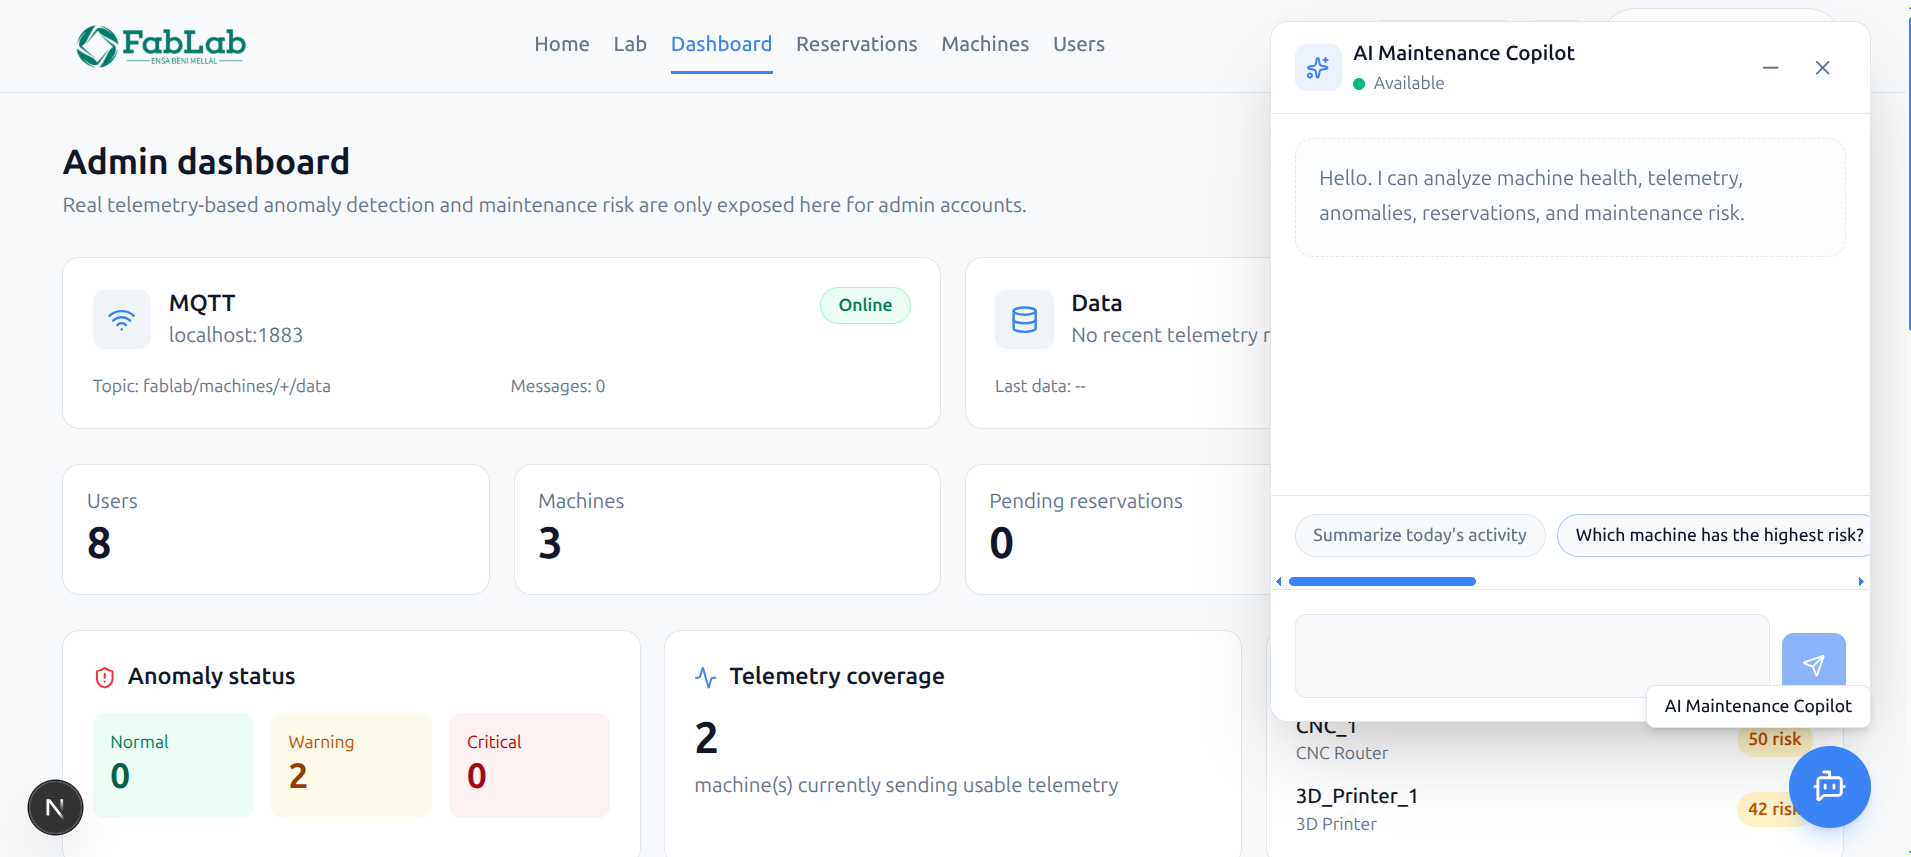
\includegraphics[width=0.82\textwidth]{images/screenshot_copilot_interface.png}}
{\fbox{\parbox[c][5cm][c]{0.82\textwidth}{\centering Emplacement réservé pour l'interface flottante du Copilote IA\\\texttt{images/screenshot\_copilot\_interface.png}}}}
\caption{Interface flottante du Copilote IA de maintenance}
\label{fig:screenshot-copilot-interface}
\end{figure}

\section{Évaluation et validation}

Les métriques disponibles concernent le classifieur NLP d'intentions. Le fichier de rapport du classifieur indique un jeu enrichi de 400 questions étiquetées, équilibrées sur 10 intentions avec 40 exemples par intention. Ce jeu est séparé en 280 exemples d'entraînement, 60 exemples de validation et 60 exemples de test.

\begin{table}[H]
\centering
\small
\caption{Métriques disponibles pour la classification NLP des intentions}
\label{tab:metrics-nlp-intents}
\begin{tabular}{|p{0.32\textwidth}|p{0.25\textwidth}|p{0.25\textwidth}|}
\hline
\rowcolor{SectionColor!12}
\textbf{Métrique} & \textbf{Validation} & \textbf{Test} \\
\hline
Accuracy & 0,6833 & 0,8333 \\
\hline
Précision macro & 0,7278 & 0,8452 \\
\hline
Rappel macro & 0,6833 & 0,8333 \\
\hline
F1-score macro & 0,6793 & 0,8355 \\
\hline
Taille de l'échantillon & 60 & 60 \\
\hline
\end{tabular}
\end{table}

Ces résultats doivent être interprétés avec prudence, car le jeu de test reste limité et provient du même corpus annoté. Ils montrent toutefois que l'enrichissement des formulations améliore nettement la classification tout en conservant le même pipeline TF-IDF et Logistic Regression.

L'évaluation actuelle du module Data Science et IA porte principalement sur le comportement en inférence, la cohérence des sorties produites, l'intégration dans la plateforme et les métriques disponibles pour le classifieur NLP. Cette validation permet de vérifier le fonctionnement global du prototype et la bonne exploitation des données simulées. Une validation quantitative plus large, appuyée sur des jeux de test indépendants et sur des données réelles, constitue toutefois une étape complémentaire nécessaire pour apprécier plus finement la robustesse des modèles dans un contexte opérationnel.

\begin{table}[H]
\centering
\small
\caption{Synthèse de l'évaluation du module Data Science et IA}
\label{tab:synthese-evaluation-ds-ia}
\begin{tabular}{|>{\raggedright\arraybackslash}p{0.30\textwidth}|>{\raggedright\arraybackslash}p{0.30\textwidth}|>{\raggedright\arraybackslash}p{0.30\textwidth}|}
\hline
\rowcolor{SectionColor!12}
\textbf{Composant} & \textbf{Validation réalisée} & \textbf{Validation complémentaire proposée} \\
\hline
Isolation Forest & Chargement du modèle, production du score d'anomalie, tests d'inférence et intégration dans la plateforme. & Validation sur données réelles, étude de stabilité et comparaison avec des scénarios connus. \\
\hline
Random Forest & Vérification des variables d'entrée, des classes et des prédictions produites. & Évaluation quantitative sur un jeu de test indépendant et plus large. \\
\hline
Classifieur NLP & Accuracy, précision, rappel, F1-score et matrice de confusion sur le corpus enrichi. & Validation sur un jeu indépendant et davantage de questions réelles. \\
\hline
Copilote IA & Tests d'accès administrateur, classification d'intentions, extraction d'entités et génération de réponses fondées sur les données. & Évaluation utilisateur et analyse qualitative des réponses. \\
\hline
\end{tabular}
\end{table}

\section{Limites}

Les limites principales du module sont liées à la nature des données et au périmètre du prototype. La télémétrie est simulée, ce qui permet de tester les flux et les interfaces, mais ne remplace pas une collecte issue de capteurs installés sur des machines réelles. Les modèles entraînés ne sont donc pas validés industriellement.

Le jeu de données NLP a été enrichi et équilibré, ce qui améliore les métriques disponibles. Il reste toutefois limité au périmètre des intentions supportées par le backend et doit être consolidé par des questions réelles collectées en usage. Le système fonctionne comme un classifieur d'intentions supervisé, pas comme un agent conversationnel génératif. Les réponses sont déterministes et fondées sur les données disponibles.

Enfin, les recommandations doivent être comprises comme une aide à la décision. Elles distinguent les faits observés, les scores inférés et les actions conseillées, sans prétendre diagnostiquer avec certitude une panne mécanique ou électrique.

\section{Conclusion du chapitre}

Ce chapitre a isolé la contribution Data Science et IA du projet Virtual FabLab. Le module combine l'ingestion de données MQTT simulées, l'extraction de caractéristiques, la détection d'anomalies par Isolation Forest, l'estimation du risque par Random Forest, la classification supervisée des intentions par TF-IDF et Logistic Regression, ainsi qu'un Copilote IA de maintenance réservé aux administrateurs.

L'ensemble constitue une couche d'aide à la décision adaptée à un prototype académique. Les résultats doivent cependant rester contextualisés : les données sont simulées, les métriques Machine Learning industrielles sont absentes pour les modèles de maintenance, et une validation future sur données réelles reste nécessaire.
